% Important: If latex complains about unicode characters,
% please use "\usepackage[utf8x]{inputenc}" in your preamble
% You can change the size of the picture by putting it into the construct:
% 1) \resizebox{10cm}{!}{"below picture"} to scale horizontally to 10 cm
% 2) \resizebox{!}{15cm}{"below picture"} to scale vertically to 15 cm
% 3) \resizebox{10cm}{15cm}{"below picture"} a combination of above two
% It is not recomended to use the scale option of the tikzpicture environment.
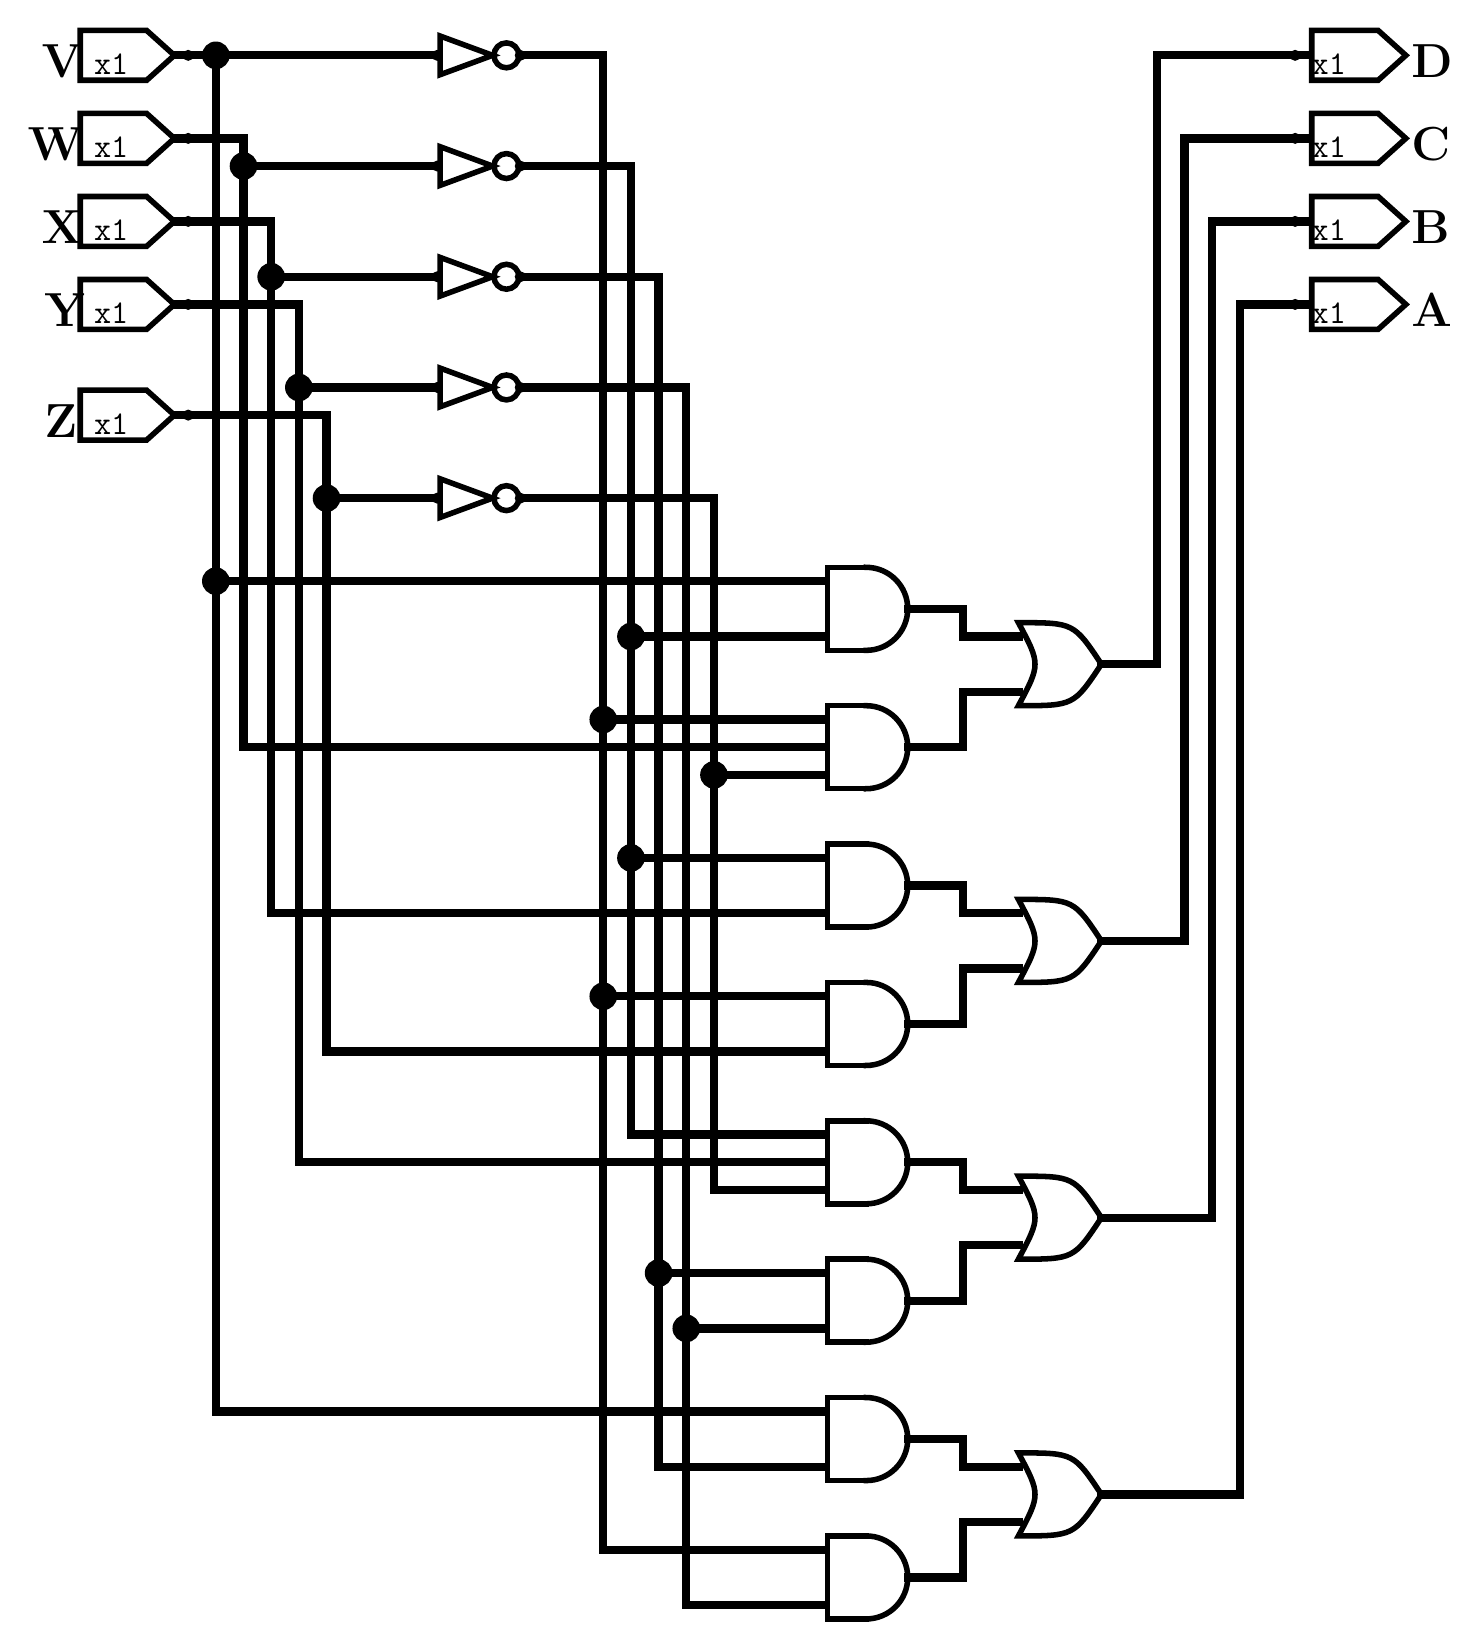
\begin{tikzpicture}[x=1pt,y=-1pt,line cap=rect]
\def\logisimfontA#1{\fontfamily{cmr}{#1}} % Replaced by logisim, original font was "SansSerif"
\def\logisimfontB#1{\fontfamily{cmtt}{#1}} % Replaced by logisim, original font was "Monospaced"
\definecolor{custcol_0_0_0}{RGB}{0, 0, 0}
\definecolor{custcol_ff_ff_ff}{RGB}{255, 255, 255}
\draw [line width=3.0pt, custcol_0_0_0 ]  (153.0,135.0) -- (103.0,135.0) -- (103.0,415.0) -- (293.0,415.0) ;
\draw [line width=3.0pt, custcol_0_0_0 ]  (293.0,375.0) -- (113.0,375.0) -- (113.0,175.0) -- (153.0,175.0) ;
\draw [line width=3.0pt, custcol_0_0_0 ]  (183.0,95.0) -- (233.0,95.0) -- (233.0,455.0) ;
\draw [line width=3.0pt, custcol_0_0_0 ]  (293.0,205.0) -- (73.0,205.0) -- (73.0,505.0) -- (293.0,505.0) ;
\draw [line width=3.0pt, custcol_0_0_0 ]  (153.0,95.0) -- (93.0,95.0) -- (93.0,325.0) -- (293.0,325.0) ;
\draw [line width=3.0pt, custcol_0_0_0 ]  (223.0,225.0) -- (293.0,225.0) ;
\draw [line width=3.0pt, custcol_0_0_0 ]  (223.0,305.0) -- (293.0,305.0) ;
\draw [line width=3.0pt, custcol_0_0_0 ]  (293.0,455.0) -- (233.0,455.0) -- (233.0,525.0) -- (293.0,525.0) ;
\draw [line width=3.0pt, custcol_0_0_0 ]  (393.0,235.0) -- (413.0,235.0) -- (413.0,15.0) -- (463.0,15.0) ;
\draw [line width=3.0pt, custcol_0_0_0 ]  (183.0,135.0) -- (243.0,135.0) -- (243.0,475.0) -- (293.0,475.0) ;
\draw [line width=3.0pt, custcol_0_0_0 ]  (183.0,55.0) -- (223.0,55.0) -- (223.0,225.0) -- (223.0,305.0) -- (223.0,405.0) -- (293.0,405.0) ;
\draw [line width=3.0pt, custcol_0_0_0 ]  (253.0,275.0) -- (253.0,425.0) -- (293.0,425.0) ;
\draw [line width=3.0pt, custcol_0_0_0 ]  (243.0,475.0) -- (243.0,575.0) -- (293.0,575.0) ;
\draw [line width=3.0pt, custcol_0_0_0 ]  (463.0,45.0) -- (423.0,45.0) -- (423.0,335.0) -- (393.0,335.0) ;
\draw [line width=3.0pt, custcol_0_0_0 ]  (393.0,435.0) -- (433.0,435.0) -- (433.0,75.0) -- (463.0,75.0) ;
\draw [line width=3.0pt, custcol_0_0_0 ]  (463.0,105.0) -- (443.0,105.0) -- (443.0,535.0) -- (393.0,535.0) ;
\draw [line width=3.0pt, custcol_0_0_0 ]  (213.0,255.0) -- (293.0,255.0) ;
\draw [line width=3.0pt, custcol_0_0_0 ]  (213.0,355.0) -- (293.0,355.0) ;
\draw [line width=3.0pt, custcol_0_0_0 ]  (183.0,15.0) -- (213.0,15.0) -- (213.0,255.0) -- (213.0,355.0) -- (213.0,555.0) -- (293.0,555.0) ;
\draw [line width=3.0pt, custcol_0_0_0 ]  (183.0,175.0) -- (253.0,175.0) -- (253.0,275.0) -- (293.0,275.0) ;
\draw [line width=3.0pt, custcol_0_0_0 ]  (83.0,55.0) -- (153.0,55.0) ;
\draw [line width=3.0pt, custcol_0_0_0 ]  (73.0,15.0) -- (73.0,205.0) ;
\fill [line width=3.0pt, custcol_0_0_0]  (113.0,175.0) ellipse (5.0 and 5.0 );
\fill [line width=3.0pt, custcol_0_0_0]  (93.0,95.0) ellipse (5.0 and 5.0 );
\fill [line width=3.0pt, custcol_0_0_0]  (73.0,205.0) ellipse (5.0 and 5.0 );
\fill [line width=3.0pt, custcol_0_0_0]  (253.0,275.0) ellipse (5.0 and 5.0 );
\fill [line width=3.0pt, custcol_0_0_0]  (213.0,255.0) ellipse (5.0 and 5.0 );
\fill [line width=3.0pt, custcol_0_0_0]  (223.0,225.0) ellipse (5.0 and 5.0 );
\fill [line width=3.0pt, custcol_0_0_0]  (73.0,15.0) ellipse (5.0 and 5.0 );
\fill [line width=3.0pt, custcol_0_0_0]  (233.0,455.0) ellipse (5.0 and 5.0 );
\fill [line width=3.0pt, custcol_0_0_0]  (103.0,135.0) ellipse (5.0 and 5.0 );
\fill [line width=3.0pt, custcol_0_0_0]  (213.0,355.0) ellipse (5.0 and 5.0 );
\fill [line width=3.0pt, custcol_0_0_0]  (223.0,305.0) ellipse (5.0 and 5.0 );
\fill [line width=3.0pt, custcol_0_0_0]  (83.0,55.0) ellipse (5.0 and 5.0 );
\fill [line width=3.0pt, custcol_0_0_0]  (243.0,475.0) ellipse (5.0 and 5.0 );
\draw [line width=3.0pt, custcol_0_0_0 ]  (58.0,75.0) -- (63.0,75.0) -- (93.0,75.0) -- (93.0,95.0) ;
\draw [line width=2.0pt, custcol_0_0_0 ]  (48.0,84.0) -- (58.0,75.0) -- (48.0,66.0) -- (24.0,66.0) -- (24.0,84.0) -- cycle;
\logisimfontB{\fontsize{12pt}{12pt}\selectfont\node[inner sep=0, outer sep=0, custcol_0_0_0, anchor=base west] at  (29.0,82.0)  {x1};}
\logisimfontA{\fontsize{16pt}{16pt}\fontseries{bx}\selectfont\node[inner sep=0, outer sep=0, custcol_0_0_0, anchor=base west] at  (10.0,83.0)  {X};}
\fill [line width=2.0pt, custcol_0_0_0]  (63.0,75.0) ellipse (2.0 and 2.0 );
\draw [line width=3.0pt, custcol_0_0_0 ]  (58.0,105.0) -- (63.0,105.0) -- (103.0,105.0) -- (103.0,135.0) ;
\draw [line width=2.0pt, custcol_0_0_0 ]  (48.0,114.0) -- (58.0,105.0) -- (48.0,96.0) -- (24.0,96.0) -- (24.0,114.0) -- cycle;
\logisimfontB{\fontsize{12pt}{12pt}\selectfont\node[inner sep=0, outer sep=0, custcol_0_0_0, anchor=base west] at  (29.0,112.0)  {x1};}
\logisimfontA{\fontsize{16pt}{16pt}\fontseries{bx}\selectfont\node[inner sep=0, outer sep=0, custcol_0_0_0, anchor=base west] at  (11.0,113.0)  {Y};}
\fill [line width=2.0pt, custcol_0_0_0]  (63.0,105.0) ellipse (2.0 and 2.0 );
\draw [line width=3.0pt, custcol_0_0_0 ]  (58.0,145.0) -- (63.0,145.0) -- (113.0,145.0) -- (113.0,175.0) ;
\draw [line width=2.0pt, custcol_0_0_0 ]  (48.0,154.0) -- (58.0,145.0) -- (48.0,136.0) -- (24.0,136.0) -- (24.0,154.0) -- cycle;
\logisimfontB{\fontsize{12pt}{12pt}\selectfont\node[inner sep=0, outer sep=0, custcol_0_0_0, anchor=base west] at  (29.0,152.0)  {x1};}
\logisimfontA{\fontsize{16pt}{16pt}\fontseries{bx}\selectfont\node[inner sep=0, outer sep=0, custcol_0_0_0, anchor=base west] at  (11.0,153.0)  {Z};}
\fill [line width=2.0pt, custcol_0_0_0]  (63.0,145.0) ellipse (2.0 and 2.0 );
\draw [line width=3.0pt, custcol_0_0_0 ]  (58.0,15.0) -- (63.0,15.0) -- (73.0,15.0) -- (153.0,15.0) ;
\draw [line width=2.0pt, custcol_0_0_0 ]  (48.0,24.0) -- (58.0,15.0) -- (48.0,6.0) -- (24.0,6.0) -- (24.0,24.0) -- cycle;
\logisimfontB{\fontsize{12pt}{12pt}\selectfont\node[inner sep=0, outer sep=0, custcol_0_0_0, anchor=base west] at  (29.0,22.0)  {x1};}
\logisimfontA{\fontsize{16pt}{16pt}\fontseries{bx}\selectfont\node[inner sep=0, outer sep=0, custcol_0_0_0, anchor=base west] at  (10.0,23.0)  {V};}
\fill [line width=2.0pt, custcol_0_0_0]  (63.0,15.0) ellipse (2.0 and 2.0 );
\draw [line width=3.0pt, custcol_0_0_0 ]  (58.0,45.0) -- (63.0,45.0) -- (83.0,45.0) -- (83.0,55.0) -- (83.0,265.0) -- (293.0,265.0) ;
\draw [line width=2.0pt, custcol_0_0_0 ]  (48.0,54.0) -- (58.0,45.0) -- (48.0,36.0) -- (24.0,36.0) -- (24.0,54.0) -- cycle;
\logisimfontB{\fontsize{12pt}{12pt}\selectfont\node[inner sep=0, outer sep=0, custcol_0_0_0, anchor=base west] at  (29.0,52.0)  {x1};}
\logisimfontA{\fontsize{16pt}{16pt}\fontseries{bx}\selectfont\node[inner sep=0, outer sep=0, custcol_0_0_0, anchor=base west] at  (5.0,53.0)  {W};}
\fill [line width=2.0pt, custcol_0_0_0]  (63.0,45.0) ellipse (2.0 and 2.0 );
\draw [line width=3.0pt, custcol_0_0_0 ]  (467.0,75.0) -- (464.0,75.0) ;
\draw [line width=2.0pt, custcol_0_0_0 ]  (493.0,66.0) -- (503.0,75.0) -- (493.0,84.0) -- (469.0,84.0) -- (469.0,66.0) -- cycle;
\logisimfontB{\fontsize{12pt}{12pt}\selectfont\node[inner sep=0, outer sep=0, custcol_0_0_0, anchor=base west] at  (469.0,82.0)  {x1};}
\logisimfontA{\fontsize{16pt}{16pt}\fontseries{bx}\selectfont\node[inner sep=0, outer sep=0, custcol_0_0_0, anchor=base west] at  (505.0,83.0)  {B};}
\fill [line width=2.0pt, custcol_0_0_0]  (463.0,75.0) ellipse (2.0 and 2.0 );
\draw [line width=3.0pt, custcol_0_0_0 ]  (467.0,105.0) -- (464.0,105.0) ;
\draw [line width=2.0pt, custcol_0_0_0 ]  (493.0,96.0) -- (503.0,105.0) -- (493.0,114.0) -- (469.0,114.0) -- (469.0,96.0) -- cycle;
\logisimfontB{\fontsize{12pt}{12pt}\selectfont\node[inner sep=0, outer sep=0, custcol_0_0_0, anchor=base west] at  (469.0,112.0)  {x1};}
\logisimfontA{\fontsize{16pt}{16pt}\fontseries{bx}\selectfont\node[inner sep=0, outer sep=0, custcol_0_0_0, anchor=base west] at  (505.0,113.0)  {A};}
\fill [line width=2.0pt, custcol_0_0_0]  (463.0,105.0) ellipse (2.0 and 2.0 );
\draw [line width=3.0pt, custcol_0_0_0 ]  (467.0,15.0) -- (464.0,15.0) ;
\draw [line width=2.0pt, custcol_0_0_0 ]  (493.0,6.0) -- (503.0,15.0) -- (493.0,24.0) -- (469.0,24.0) -- (469.0,6.0) -- cycle;
\logisimfontB{\fontsize{12pt}{12pt}\selectfont\node[inner sep=0, outer sep=0, custcol_0_0_0, anchor=base west] at  (469.0,22.0)  {x1};}
\logisimfontA{\fontsize{16pt}{16pt}\fontseries{bx}\selectfont\node[inner sep=0, outer sep=0, custcol_0_0_0, anchor=base west] at  (505.0,23.0)  {D};}
\fill [line width=2.0pt, custcol_0_0_0]  (463.0,15.0) ellipse (2.0 and 2.0 );
\draw [line width=3.0pt, custcol_0_0_0 ]  (467.0,45.0) -- (464.0,45.0) ;
\draw [line width=2.0pt, custcol_0_0_0 ]  (493.0,36.0) -- (503.0,45.0) -- (493.0,54.0) -- (469.0,54.0) -- (469.0,36.0) -- cycle;
\logisimfontB{\fontsize{12pt}{12pt}\selectfont\node[inner sep=0, outer sep=0, custcol_0_0_0, anchor=base west] at  (469.0,52.0)  {x1};}
\logisimfontA{\fontsize{16pt}{16pt}\fontseries{bx}\selectfont\node[inner sep=0, outer sep=0, custcol_0_0_0, anchor=base west] at  (505.0,53.0)  {C};}
\fill [line width=2.0pt, custcol_0_0_0]  (463.0,45.0) ellipse (2.0 and 2.0 );
\draw [line width=2.0pt, custcol_0_0_0 ]  (173.0,55.0) -- (154.0,48.0) -- (154.0,62.0) -- cycle;
\draw [line width=2.0pt, custcol_0_0_0]  (178.0,55.0) ellipse (4.5 and 4.5 );
\fill [line width=2.0pt, custcol_0_0_0]  (183.0,55.0) ellipse (2.0 and 2.0 );
\fill [line width=2.0pt, custcol_0_0_0]  (153.0,55.0) ellipse (2.0 and 2.0 );
\draw [line width=2.0pt, custcol_0_0_0 ]  (173.0,95.0) -- (154.0,88.0) -- (154.0,102.0) -- cycle;
\draw [line width=2.0pt, custcol_0_0_0]  (178.0,95.0) ellipse (4.5 and 4.5 );
\fill [line width=2.0pt, custcol_0_0_0]  (183.0,95.0) ellipse (2.0 and 2.0 );
\fill [line width=2.0pt, custcol_0_0_0]  (153.0,95.0) ellipse (2.0 and 2.0 );
\draw [line width=2.0pt, custcol_0_0_0 ]  (173.0,135.0) -- (154.0,128.0) -- (154.0,142.0) -- cycle;
\draw [line width=2.0pt, custcol_0_0_0]  (178.0,135.0) ellipse (4.5 and 4.5 );
\fill [line width=2.0pt, custcol_0_0_0]  (183.0,135.0) ellipse (2.0 and 2.0 );
\fill [line width=2.0pt, custcol_0_0_0]  (153.0,135.0) ellipse (2.0 and 2.0 );
\draw [line width=2.0pt, custcol_0_0_0 ]  (173.0,175.0) -- (154.0,168.0) -- (154.0,182.0) -- cycle;
\draw [line width=2.0pt, custcol_0_0_0]  (178.0,175.0) ellipse (4.5 and 4.5 );
\fill [line width=2.0pt, custcol_0_0_0]  (183.0,175.0) ellipse (2.0 and 2.0 );
\fill [line width=2.0pt, custcol_0_0_0]  (153.0,175.0) ellipse (2.0 and 2.0 );
\draw [line width=2.0pt, custcol_0_0_0 ]  (173.0,15.0) -- (154.0,8.0) -- (154.0,22.0) -- cycle;
\draw [line width=2.0pt, custcol_0_0_0]  (178.0,15.0) ellipse (4.5 and 4.5 );
\fill [line width=2.0pt, custcol_0_0_0]  (183.0,15.0) ellipse (2.0 and 2.0 );
\fill [line width=2.0pt, custcol_0_0_0]  (153.0,15.0) ellipse (2.0 and 2.0 );
\draw [line width=2.0pt, custcol_0_0_0] (308.0,230.0) arc (90.0:-90.0:15.0 and 15.0 );
\draw [line width=2.0pt, custcol_0_0_0 ]  (308.0,200.0) -- (294.0,200.0) -- (294.0,230.0) -- (308.0,230.0) ;
\draw [line width=2.0pt, custcol_0_0_0] (308.0,280.0) arc (90.0:-90.0:15.0 and 15.0 );
\draw [line width=2.0pt, custcol_0_0_0 ]  (308.0,250.0) -- (294.0,250.0) -- (294.0,280.0) -- (308.0,280.0) ;
\draw [line width=2.0pt, custcol_0_0_0] (308.0,330.0) arc (90.0:-90.0:15.0 and 15.0 );
\draw [line width=2.0pt, custcol_0_0_0 ]  (308.0,300.0) -- (294.0,300.0) -- (294.0,330.0) -- (308.0,330.0) ;
\draw [line width=2.0pt, custcol_0_0_0] (308.0,380.0) arc (90.0:-90.0:15.0 and 15.0 );
\draw [line width=2.0pt, custcol_0_0_0 ]  (308.0,350.0) -- (294.0,350.0) -- (294.0,380.0) -- (308.0,380.0) ;
\draw [line width=2.0pt, custcol_0_0_0] (308.0,430.0) arc (90.0:-90.0:15.0 and 15.0 );
\draw [line width=2.0pt, custcol_0_0_0 ]  (308.0,400.0) -- (294.0,400.0) -- (294.0,430.0) -- (308.0,430.0) ;
\draw [line width=2.0pt, custcol_0_0_0] (308.0,480.0) arc (90.0:-90.0:15.0 and 15.0 );
\draw [line width=2.0pt, custcol_0_0_0 ]  (308.0,450.0) -- (294.0,450.0) -- (294.0,480.0) -- (308.0,480.0) ;
\draw [line width=2.0pt, custcol_0_0_0] (308.0,530.0) arc (90.0:-90.0:15.0 and 15.0 );
\draw [line width=2.0pt, custcol_0_0_0 ]  (308.0,500.0) -- (294.0,500.0) -- (294.0,530.0) -- (308.0,530.0) ;
\draw [line width=2.0pt, custcol_0_0_0] (308.0,580.0) arc (90.0:-90.0:15.0 and 15.0 );
\draw [line width=2.0pt, custcol_0_0_0 ]  (308.0,550.0) -- (294.0,550.0) -- (294.0,580.0) -- (308.0,580.0) ;
\draw [line width=3.0pt, custcol_0_0_0 ]  (323.0,215.0) -- (343.0,215.0) -- (343.0,225.0) -- (363.0,225.0) -- (363.0,225.0) ;
\draw [line width=3.0pt, custcol_0_0_0 ]  (363.0,245.0) -- (363.0,245.0) -- (343.0,245.0) -- (343.0,265.0) -- (323.0,265.0) ;
\draw [line width=2.0pt, custcol_0_0_0 ]  (393.0,235.0) .. controls  (383.0,220.0)  ..  (363.0,220.0) .. controls  (371.0,235.0)  ..  (363.0,250.0) .. controls  (383.0,250.0)  ..  (393.0,235.0) -- cycle ;
\draw [line width=3.0pt, custcol_0_0_0 ]  (323.0,315.0) -- (343.0,315.0) -- (343.0,325.0) -- (363.0,325.0) -- (363.0,325.0) ;
\draw [line width=3.0pt, custcol_0_0_0 ]  (363.0,345.0) -- (363.0,345.0) -- (343.0,345.0) -- (343.0,365.0) -- (323.0,365.0) ;
\draw [line width=2.0pt, custcol_0_0_0 ]  (393.0,335.0) .. controls  (383.0,320.0)  ..  (363.0,320.0) .. controls  (371.0,335.0)  ..  (363.0,350.0) .. controls  (383.0,350.0)  ..  (393.0,335.0) -- cycle ;
\draw [line width=3.0pt, custcol_0_0_0 ]  (323.0,415.0) -- (343.0,415.0) -- (343.0,425.0) -- (363.0,425.0) -- (363.0,425.0) ;
\draw [line width=3.0pt, custcol_0_0_0 ]  (363.0,445.0) -- (363.0,445.0) -- (343.0,445.0) -- (343.0,465.0) -- (323.0,465.0) ;
\draw [line width=2.0pt, custcol_0_0_0 ]  (393.0,435.0) .. controls  (383.0,420.0)  ..  (363.0,420.0) .. controls  (371.0,435.0)  ..  (363.0,450.0) .. controls  (383.0,450.0)  ..  (393.0,435.0) -- cycle ;
\draw [line width=3.0pt, custcol_0_0_0 ]  (323.0,515.0) -- (343.0,515.0) -- (343.0,525.0) -- (363.0,525.0) -- (363.0,525.0) ;
\draw [line width=3.0pt, custcol_0_0_0 ]  (363.0,545.0) -- (363.0,545.0) -- (343.0,545.0) -- (343.0,565.0) -- (323.0,565.0) ;
\draw [line width=2.0pt, custcol_0_0_0 ]  (393.0,535.0) .. controls  (383.0,520.0)  ..  (363.0,520.0) .. controls  (371.0,535.0)  ..  (363.0,550.0) .. controls  (383.0,550.0)  ..  (393.0,535.0) -- cycle ;
\end{tikzpicture}

